\documentclass{ctexart}
\usepackage{geometry}
\usepackage{fancyhdr}
\usepackage{graphicx}
\usepackage{booktabs}
\usepackage{amsmath}
\usepackage{multirow}
\usepackage{tikz}
\usepackage{array}
\xeCJKsetup{CJKmath=true} 
\usepackage{zhnumber} % change section number to chinese
\renewcommand\thesection{\zhnum{section}}
\renewcommand \thesubsection {\arabic{subsection}}
\CTEXsetup[format={\Large\bfseries}]{section}

\geometry{
    a4paper,
    left=3.18cm,
    right=3.18cm,
    top=3.04cm,
    bottom=3.04cm
}

\pagestyle{fancy}
\fancyhf{}
\renewcommand{\headrulewidth}{0.7pt} % 设置页眉横线粗细
\fancyhead[L]{\kaishu\large 大学物理实验报告} % 在左侧设置页眉文字
\fancyhead[R]{\kaishu\large 哈尔滨工业大学(深圳) } % 在右侧设置页眉文字
\fancyfoot[R]{\thepage} % 将页数放在右下角


\setlength\headwidth{\textwidth}

\begin{document}

\noindent
\begin{center}
\textbf{
\begin{tabular}{p{2.4cm}p{2.4cm}p{4cm}p{4cm}}
    班级 \hrulefill & 学号 \hrulefill & 姓名 \hrulefill & 教师签字 \hrulefill \\
\end{tabular}
\begin{tabular}{p{6cm}p{3.6cm}p{3.6cm}}
    实验日期 \hrulefill & 预习成绩 \hrulefill & 总成绩 \hrulefill
\end{tabular}
{\noindent}	 \rule[-10pt]{\textwidth}{0.7pt}
}\end{center}

\begin{center}
    \Large \textbf{实验内容 \underline{用示波器观测磁滞回线}}
\end{center}

\section{实验目的}
\vspace*{6\baselineskip}
\section{预习内容}

\subsection{剩磁、矫顽力、基本磁化曲线、动态磁滞回线的定义。}
\vspace*{10\baselineskip}
\subsection{示波器测量的$X$轴信号$U_x$是谁的电压?和磁场强度$H$是什么关系(写出公式)?示波器测量的$Y$轴信号$U_y$是谁的电压?和磁感应强度$B$是什么关系(写出公式)?}
\newpage
\section{数据记录}
\textbf{样品1:饱和磁滞回线}
\begin{table}[!h]
    \renewcommand{\arraystretch}{1.2}
    \centering
    \begin{tabular}{|c|m{0.5cm}<{\centering}|m{0.5cm}<{\centering}|m{0.5cm}<{\centering}|c|m{0.5cm}<{\centering}|m{0.5cm}<{\centering}|m{0.5cm}<{\centering}|m{0.5cm}<{\centering}|m{0.5cm}<{\centering}|m{0.5cm}<{\centering}|m{0.5cm}<{\centering}|m{0.5cm}<{\centering}|m{0.5cm}<{\centering}|m{0.5cm}<{\centering}|}
        \hline
        频率 & $R_1$ & $R_2$ & $C$ & & 1 & 2 & 3 & 4 & 5 & 6 & 7 & 8 & 9 & 10 \\
        \hline
        \multirow{2}*{$50 Hz$} & \multirow{2}*{} & \multirow{2}*{} & &$U_x$ &  &  &  &  &  &  &  &  &  &  \\
        \cline{5-15}
        & &  & & $U_y$ &  &  &  &  &  &  &  &  &  &  \\
        \hline
        \multicolumn{4}{|c|}{\multirow{3}*{}} &  & 11 & 12 & 13 & 14 & 15 & 16 & 17 & 18 & 19 & 20 \\
        \cline{5-15}
        \multicolumn{4}{|c|}{} & $U_x$ &  &  &  &  &  &  &  &  &  &  \\
        \cline{5-15}
        \multicolumn{4}{|c|}{} & $U_y$ &  &  &  &  &  &  &  &  &  &  \\
        \hline
    \end{tabular}
\end{table}

\textbf{样品1:基本磁滞回线}
\begin{table}[!h]
    \renewcommand{\arraystretch}{1.2}
    \centering
    \begin{tabular}{|c|m{0.5cm}<{\centering}|m{0.5cm}<{\centering}|m{0.5cm}<{\centering}|c|m{0.5cm}<{\centering}|m{0.5cm}<{\centering}|m{0.5cm}<{\centering}|m{0.5cm}<{\centering}|m{0.5cm}<{\centering}|m{0.5cm}<{\centering}|m{0.5cm}<{\centering}|m{0.5cm}<{\centering}|m{0.5cm}<{\centering}|m{0.5cm}<{\centering}|}
        \hline
        频率 & $R_1$ & $R_2$ & $C$ & & 1 & 2 & 3 & 4 & 5 & 6 & 7 & 8 & 9 & 10 \\
        \hline
        \multirow{2}*{$50 Hz$} & \multirow{2}*{} & \multirow{2}*{} & &$U_x$ &  &  &  &  &  &  &  &  &  &  \\
        \cline{5-15}
        & &  & & $U_y$ &  &  &  &  &  &  &  &  &  &  \\
        \hline
    \end{tabular}
\end{table}

\textbf{样品2:饱和磁滞回线}
\begin{table}[!h]
    \renewcommand{\arraystretch}{1.2}
    \centering
    \begin{tabular}{|c|m{0.5cm}<{\centering}|m{0.5cm}<{\centering}|m{0.5cm}<{\centering}|c|m{0.5cm}<{\centering}|m{0.5cm}<{\centering}|m{0.5cm}<{\centering}|m{0.5cm}<{\centering}|m{0.5cm}<{\centering}|m{0.5cm}<{\centering}|m{0.5cm}<{\centering}|m{0.5cm}<{\centering}|m{0.5cm}<{\centering}|m{0.5cm}<{\centering}|}
        \hline
        频率 & $R_1$ & $R_2$ & $C$ & & 1 & 2 & 3 & 4 & 5 & 6 & 7 & 8 & 9 & 10 \\
        \hline
        \multirow{2}*{$50 Hz$} & \multirow{2}*{} & \multirow{2}*{} & &$U_x$ &  &  &  &  &  &  &  &  &  &  \\
        \cline{5-15}
        & &  & & $U_y$ &  &  &  &  &  &  &  &  &  &  \\
        \hline
        \multicolumn{4}{|c|}{\multirow{3}*{}} &  & 11 & 12 & 13 & 14 & 15 & 16 & 17 & 18 & 19 & 20 \\
        \cline{5-15}
        \multicolumn{4}{|c|}{} & $U_x$ &  &  &  &  &  &  &  &  &  &  \\
        \cline{5-15}
        \multicolumn{4}{|c|}{} & $U_y$ &  &  &  &  &  &  &  &  &  &  \\
        \hline
    \end{tabular}
\end{table}

\textbf{样品2:基本磁滞回线}
\begin{table}[!h]
    \renewcommand{\arraystretch}{1.2}
    \centering
    \begin{tabular}{|c|m{0.5cm}<{\centering}|m{0.5cm}<{\centering}|m{0.5cm}<{\centering}|c|m{0.5cm}<{\centering}|m{0.5cm}<{\centering}|m{0.5cm}<{\centering}|m{0.5cm}<{\centering}|m{0.5cm}<{\centering}|m{0.5cm}<{\centering}|m{0.5cm}<{\centering}|m{0.5cm}<{\centering}|m{0.5cm}<{\centering}|m{0.5cm}<{\centering}|}
        \hline
        频率 & $R_1$ & $R_2$ & $C$ & & 1 & 2 & 3 & 4 & 5 & 6 & 7 & 8 & 9 & 10 \\
        \hline
        \multirow{2}*{$50 Hz$} & \multirow{2}*{} & \multirow{2}*{} & &$U_x$ &  &  &  &  &  &  &  &  &  &  \\
        \cline{5-15}
        & &  & & $U_y$ &  &  &  &  &  &  &  &  &  &  \\
        \hline
    \end{tabular}
\end{table}

\begin{tikzpicture}[remember picture,overlay]
    \node[anchor=south east,inner sep=100pt] at (current page.south east) {
        \renewcommand{\arraystretch}{1.5} % 表格行高倍数
        \setlength{\tabcolsep}{18pt}    
    \begin{tabular}{|c|c|}
        \hline
        \LARGE  教师 & \LARGE  姓名 \\
        \hline
        \LARGE \kaishu 签字 &  \\
        \hline
        \end{tabular}
    };
\end{tikzpicture}

\newpage

\section{数据处理及绘图}

有理论公式:

$$ H = \frac{N_1}{L \cdot R_1} U_x $$

$$ B = \frac{R_2 \cdot C}{N_2\cdot S} U_y $$

将数据计算得到$B-H$曲线,绘制如下磁滞回线图。

\begin{figure}[!h]
    \centering
    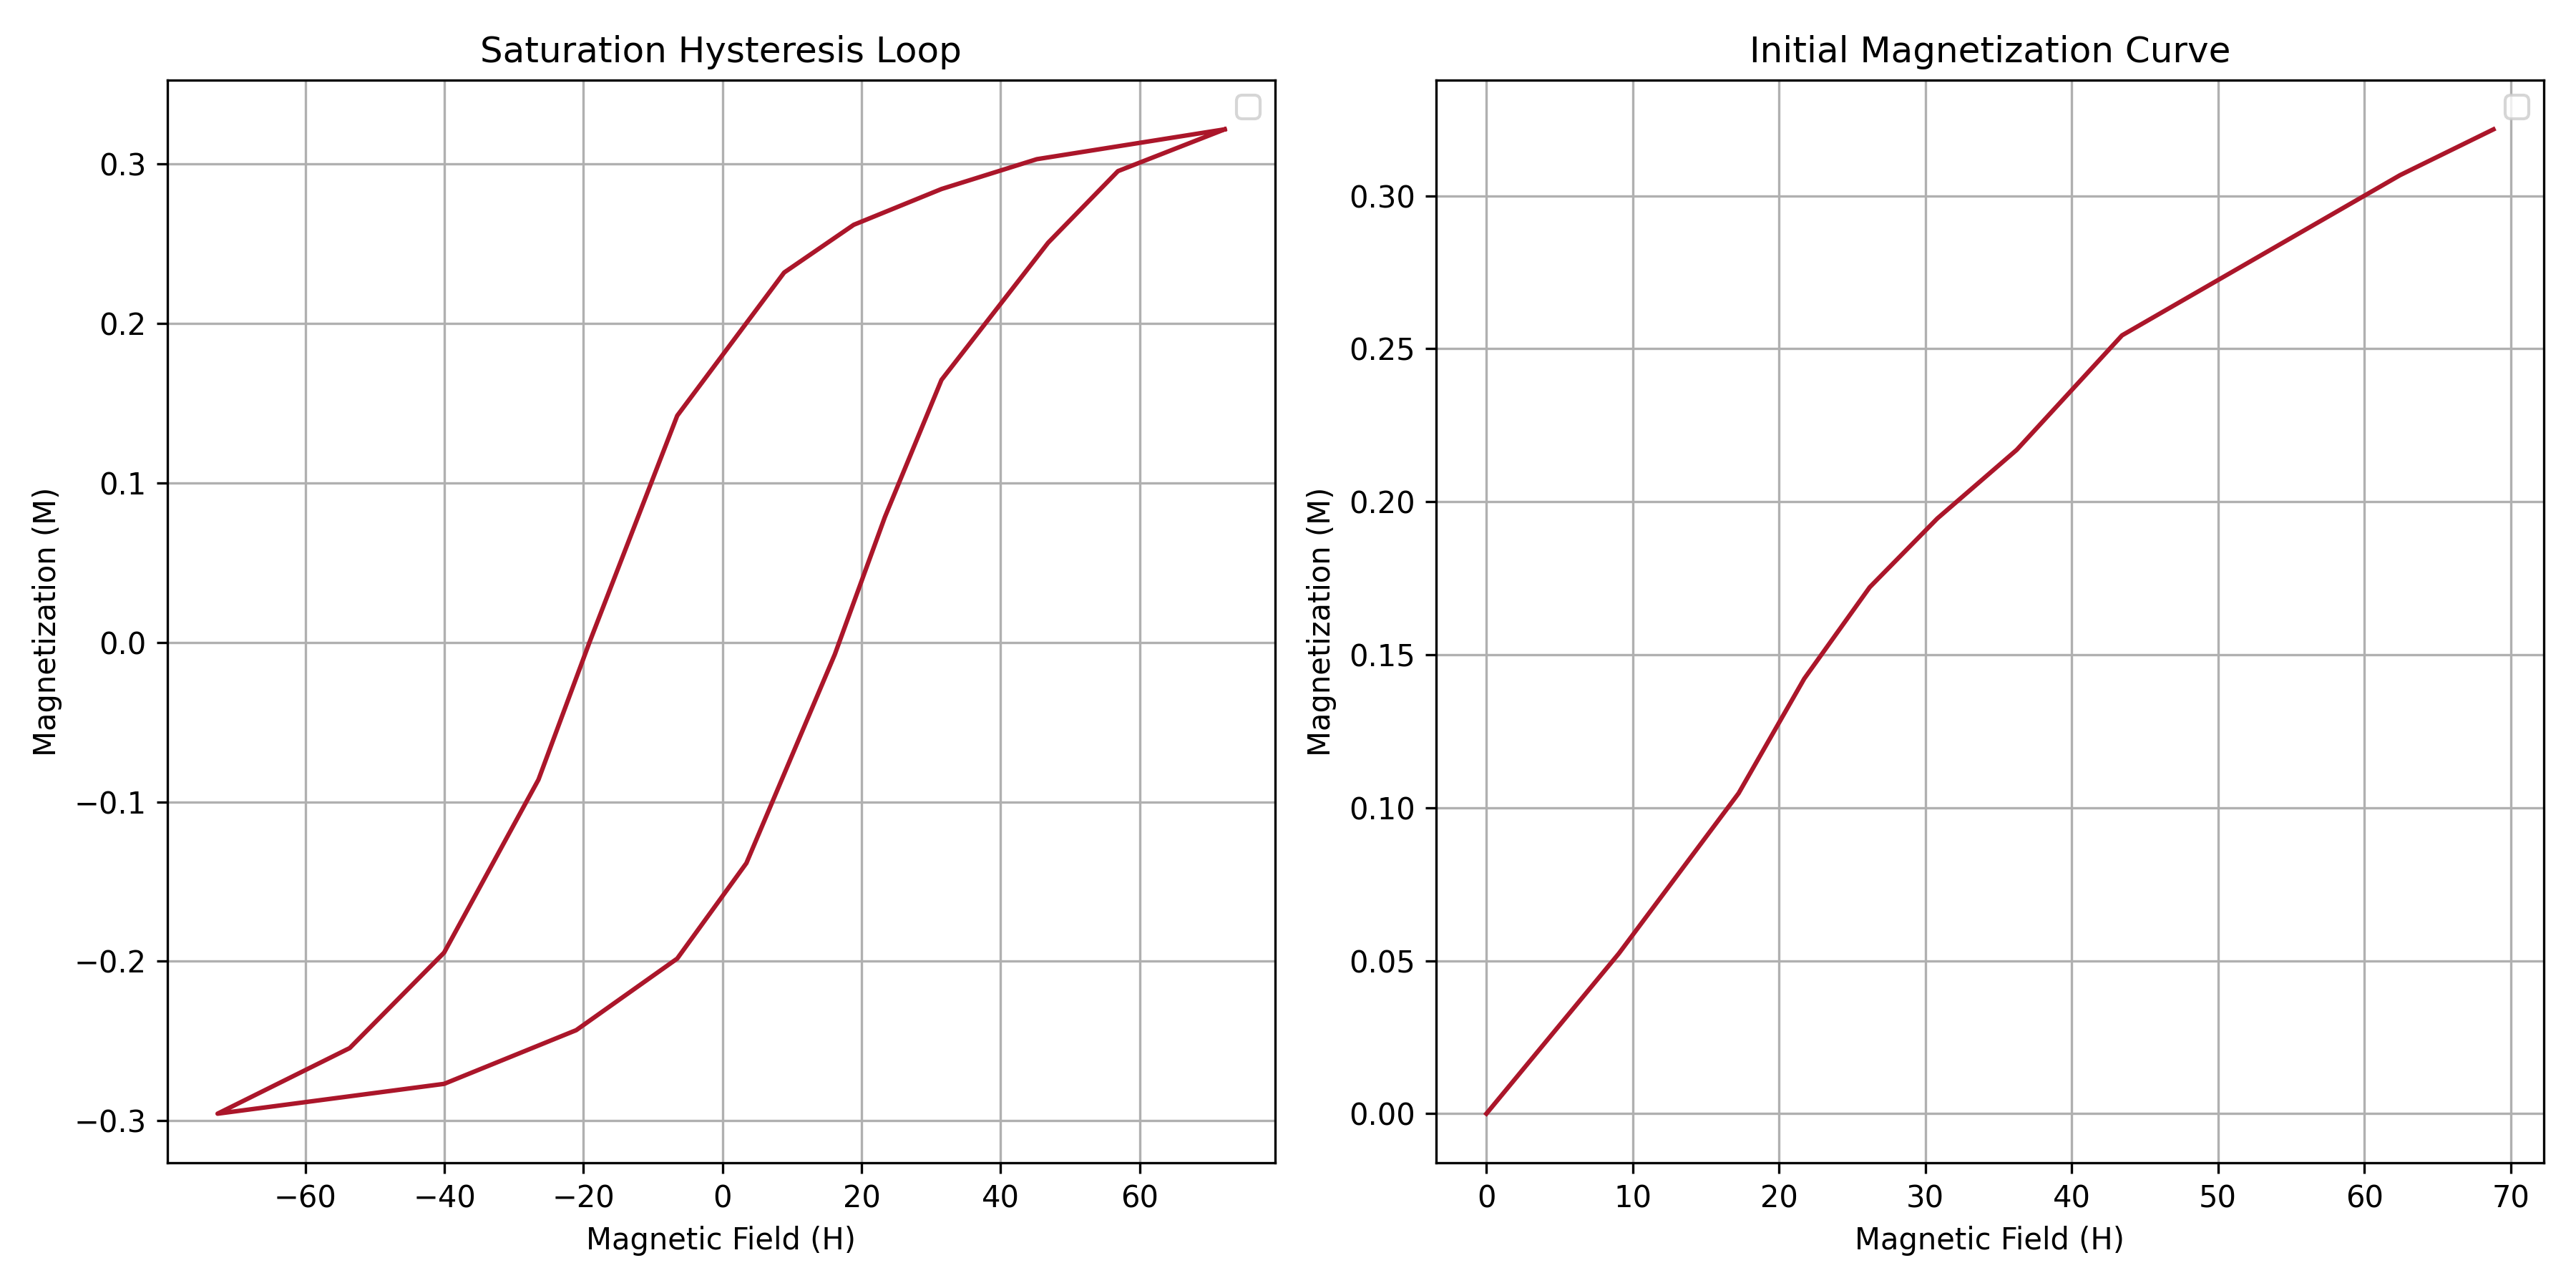
\includegraphics[width=\textwidth]{0.png}
    \caption{样品一}
\end{figure}

\begin{figure}[!h]
    \centering
    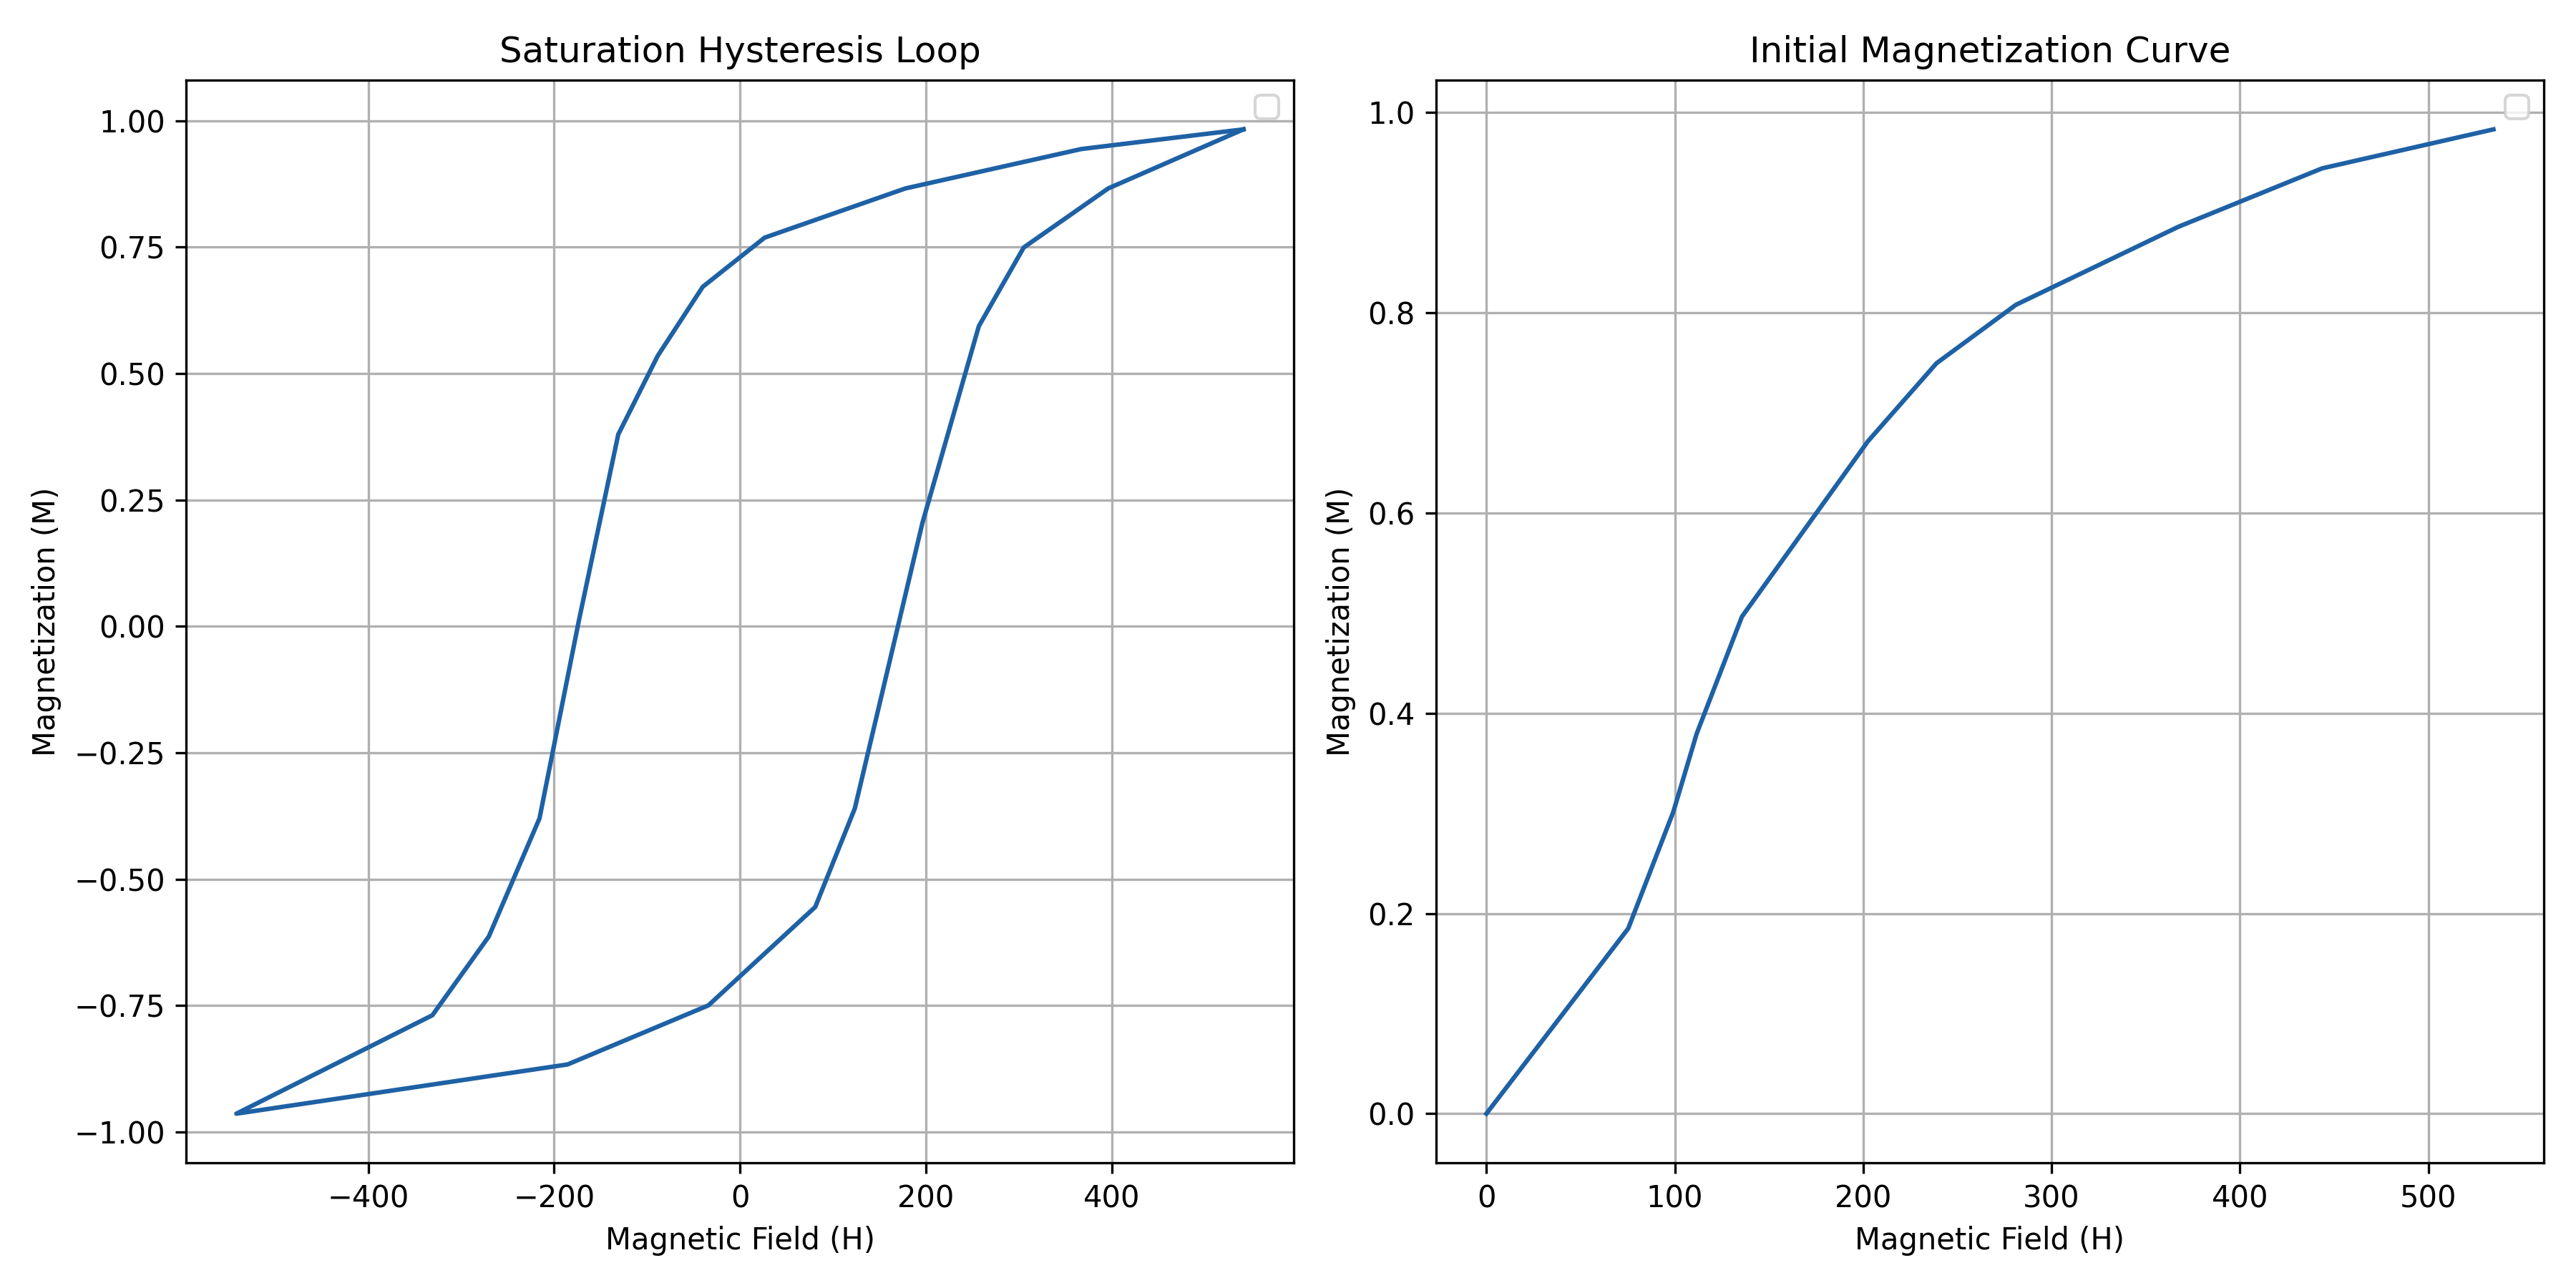
\includegraphics[width=\textwidth]{1.png}
    \caption{样品二}
\end{figure}

利用绘制的磁滞回线图,得到样品的剩磁以及矫顽力。

\begin{table}
    \renewcommand{\arraystretch}{1.2}
    \centering
    \begin{tabular}{ccc}
        \toprule
        \textbf{样品} & \textbf{剩磁} & \textbf{矫顽力} \\
        \midrule
        样品一 & $0.17 T$ & $18.6 A/m$ \\
        
        样品二 & $0.71 T$ & $171 A/m$ \\
        \bottomrule
    \end{tabular}
\end{table}

\section{讨论问题}

\subsection{某两种材料的磁滞回线,一个很宽一个很窄,它们各属于哪类磁性材料?分别可以应用于什么场合?}

很宽的是软磁材料,如铁镍合金,硅钢等等,具有较小的矫顽力和饱和磁感应强度,容易被磁化和去磁。宽磁滞回线表明材料在磁化和去磁时能量损耗较小。广泛应用于电感器、变压器、磁屏蔽和电机等领域,尤其是在需要频繁磁化和去磁的应用中。

狭窄的是硬磁材料,如钕铁硼($NdFeB$)、钴基合金等。具有较大的矫顽力和饱和磁感应强度,磁化后保持磁性,窄磁滞回线表明材料的能量损耗较大,但磁性保持性好。常用于永磁体、扬声器、磁铁、电子元件等领域,特别是在需要长时间保持磁性和较高磁场强度的应用中。

\subsection{一钢制部件不慎被磁化,请设计退磁方案。}

对于钢制部件的退磁方案,可以采用电磁退磁器进行处理。电磁退磁器通过交变电流产生交变磁场,将部件放置在设备内,启动退磁器并逐渐移动部件,以确保每个区域都能受到退磁影响。在操作过程中,电流应逐渐减小,以减少残余磁性。

对于较小或复杂的部件,可以考虑使用高频退磁器,这种设备利用高频电磁波通过材料来消除磁性。如果条件允许,可以将部件加热到居里温度以上(通常在500°C以上),然后缓慢冷却,以消除内部磁性。此外,机械振动也可以作为一种退磁方法,通过在振动台上震动部件,使内部磁畴重新排列。

手动退磁器是一种简单有效的工具,可以沿着部件表面来回移动,逐步降低与部件的距离,达到降低残余磁性的效果。在完成退磁后,使用磁性测量工具(如磁力计)检查部件的磁性是否已被完全消除,如有必要,可重复退磁过程。

\end{document}